\section{Schwingungen \kuchling{192} \stoecker{235}}
\subsection{Ungedämpfte Schwingungen}
\renewcommand{\arraystretch}{2}
\begin{tabular}{|p{4cm}|p{8cm}|p{6cm}|}
	\hline
	\begin{minipage}[]{4cm}
    	Harmonische Schwingung\\
    	\kuchling{193} \stoecker{236}\\
    \end{minipage} &
	\begin{minipage}[]{8cm}
 		$y=A\,\sin(\omega t+ \varphi)  \qquad \omega=\dfrac{2\pi}{T}=2\pi f$\\ \\
		$\ddot{y}+\omega^2y=0 \qquad v(t)=\dot{y} \qquad a(t)=\ddot{y}$
    \end{minipage} &
	\begin{minipage}[]{6cm}
        \vspace{0.2cm}
 		$A$ = Amplitude $[1]$\\
 		$\omega$ = Kreisfrequenz $[\frac{1}{s}]$\\
 		$v(t)$ = Geschwindigkeit $[\frac{m}{s}]$\\
 		$a(t)$ = Beschleunigung $[\frac{m}{s^2}]$
     \end{minipage}\\
    \begin{minipage}[]{4cm} 
        	Trägheitskraft/Moment
    \end{minipage}&    
    \begin{minipage}[]{8cm}
        	Trans. : $F_T(y) = m \cdot \ddot{y} \qquad$
        	Rot.: $M_T(\varphi) = J \cdot \ddot{\varphi}$
    \end{minipage} &
    \begin{minipage}[]{6cm}
    		$J = [kg \cdot m^2]$
    \end{minipage}\\
	\hline
	\begin{minipage}[]{4cm}
    	Schwingungsenergie\\
    	\kuchling{203} \stoecker{240}\\
    \end{minipage} &
	\begin{minipage}[]{8cm}
    \vspace{0.2cm}
	$E=E_{\text{pot}}+E_{\text{kin}}=\dfrac{c\,y^2}{2}+\dfrac{m\,v^2}{2}= \dfrac{c}{2}\cdot A$\\
	\\ $\dfrac{m\,\omega^2A^2}{2}(\sin(\omega t+\varphi)^2+\cos(\omega
	t+\varphi)^2)=\dfrac{m\,\omega^2\,A^2}{2}$\\
	\end{minipage} &
	\begin{minipage}[]{6cm}
		$E$ = Energie $[J]\\$
		$v=\dot y$ = Geschwindigkeit $[\frac{m}{s}]$\\
		$m$ = Masse $[kg]$\\	
    \end{minipage}\\
	\hline		
	\begin{minipage}[]{4cm}
    	Federpendel\\
    	\kuchling{198} \stoecker{238}\\
    \end{minipage} &
	\begin{minipage}[]{8cm}
    	\underline{ohne Federmasse:}\\
		$m\ddot{y}+c\,y=0 \qquad \omega_0=\sqrt{\dfrac{c}{m}} = \sqrt{\dfrac{c_1 +
		c_2}{m_1 + m_2}}$ \\ $T=2\pi \sqrt{\dfrac{m}{c}}$\\ \\
		rücktr. Kraft: $F=-cy=m\,\ddot{y} = F_T$ \\ \\
		\underline{mit Federmasse:}\\
		$\omega_0=\sqrt{\dfrac{c}{m+\frac{m_F}{3}}} \qquad
		T=2\pi\sqrt{\dfrac{m+\frac{m_F}{3}}{c}}$\\ 
		\end{minipage} &
	\begin{minipage}[]{6cm}
		\parbox[2cm]{4cm}{
		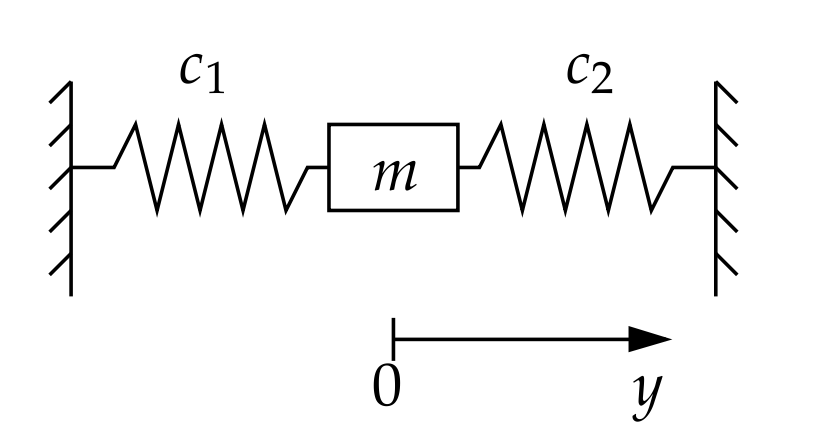
\includegraphics[width=3.5cm]{./bilder/Federpendel_masselos.png}}\\ \\
		\parbox[2cm]{4cm}{
		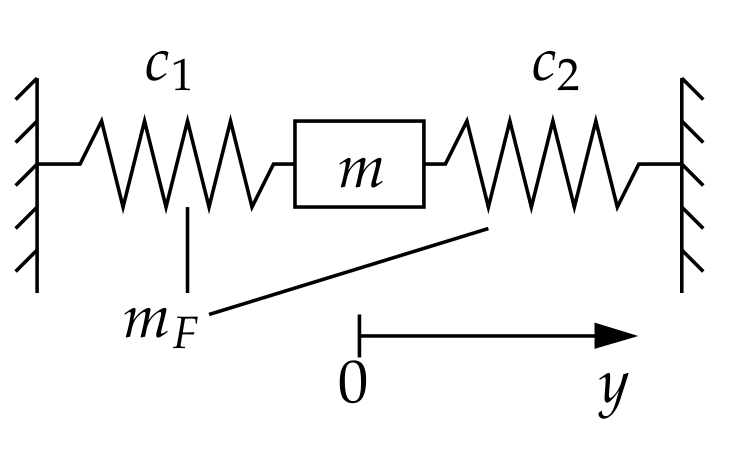
\includegraphics[width=3.5cm]{./bilder/Federpendel_masse.png}}	\\		
    \end{minipage}\\
	\hline
	\begin{minipage}[]{4cm}
    	Drehpendel\\
    	\kuchling{199} \stoecker{245}\\
    \end{minipage} &
	\begin{minipage}[]{8cm}
	$J\ddot{\varphi}+c_{_D}\varphi=0 \qquad \omega_0=\sqrt{\dfrac{c_{_D}}{J}} \qquad
	T=2\pi\sqrt{\dfrac{J}{c_{_D}}}$\\ \\
	rücktr. Drehm.:	$M=-c_{_D}\,\varphi=J\,\ddot{\varphi}$ (Bewegung)\\
	\end{minipage} &
	\begin{minipage}[]{6cm}
    	\vspace{0.1cm}
		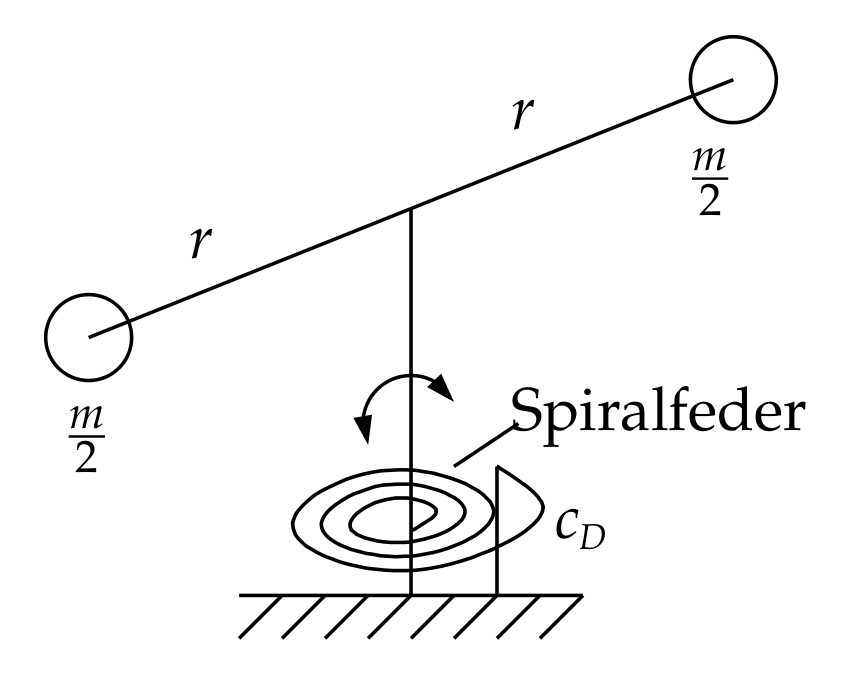
\includegraphics[width=3.5cm]{./bilder/Drehpendel.png}	
		$c_{_D} = [\frac{N \cdot m}{rad}]$
    \end{minipage}\\
	\hline
	\begin{minipage}[]{4cm}
    	Fadenpendel,\\
    	Mathematisches Pendel\\
    	\kuchling{200} \stoecker{240}\\
    \end{minipage} &
	\begin{minipage}[]{8cm}
	$l\ddot{\varphi}+g\sin(\varphi)=0\quad\xrightarrow{\text{lin.} (\varphi \ll 1)}\quad
	l\ddot{\varphi}+g\varphi=0$\\ \\
	$\omega_0=\sqrt{\dfrac{g}{l}} \qquad T=2\pi\sqrt{\dfrac{l}{g}} \qquad
	v=l\dot{\varphi} \qquad a=l\ddot{\varphi}$\\
	\end{minipage} &
	\begin{minipage}[]{6cm}
    	\vspace{0.1cm}
		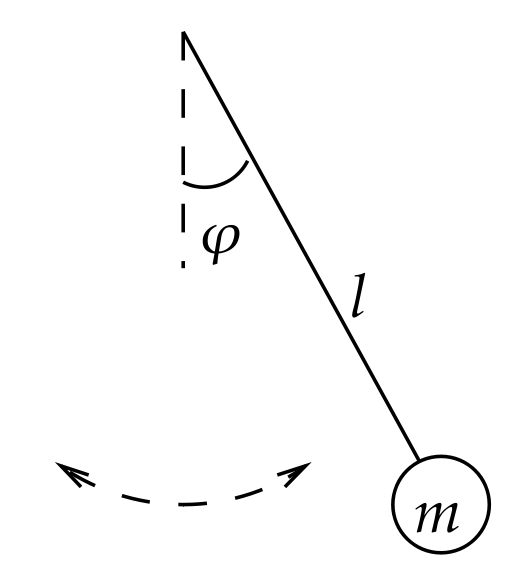
\includegraphics[width=2cm]{./bilder/mathe_pendel.png}	
    \end{minipage}\\
	\hline
	\begin{minipage}[]{4cm}
    	Physisches Pendel\\
    	\kuchling{201} \stoecker{243}\\ \\ \\
    	Massenträgheitsmomente\\
    	\kuchling{131} \stoecker{103}\\
    \end{minipage} &
	\begin{minipage}[]{8cm}
    \vspace{0.2cm}
	$J_A\ddot{\varphi}+m\,g\,a\sin(\varphi)=0$ $\xrightarrow{\text{lin.}}$ $
	J_A\ddot{\varphi}+m\,g\,a\,\varphi=0$\\ \\
	$\omega_0 = \sqrt{\dfrac{m\,g\,a}{J_A}}=\sqrt{\dfrac{g}{l^{*}}} \qquad
	T=2\pi\sqrt{\dfrac{J_A}{m\,g\,a}}=2\pi\sqrt{\dfrac{l^*}{g}}$\\ \\
	$l^{*}=\dfrac{J_A}{m\,a}=\dfrac{J_M}{m\,x} = \dfrac{J_{S}}{m\cdot a}+a$\\ 
	bei mehreren Elementen: \parbox{3cm}{
			$J_A = \sum J_{A_i}$\\
				 $m = \sum m_i$}\\ \\
	$J_A=J_S+m\,a^2 \qquad J_M=J_S+m\,x^2$\\ \\
	\textbf{Perkussionszentrum}\\
	Trifft ein Schlag den Schwingungsmittelpunkt $M$ wirken keine Kräfte auf den
	Punkt $A$ \& umgekehrt\\
	\textbf{Minimale Schwingungsdauer}\\
	$l_{min}^* = 2\sqrt{\dfrac{J_S}{m}}$ wenn $a=x=a_{min}$
	\end{minipage} &
	\begin{minipage}[]{6cm}
		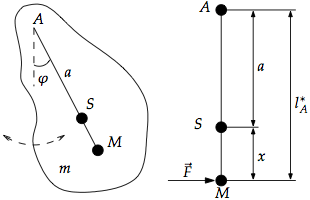
\includegraphics[width=6cm]{./bilder/physpendel.png}\\	
		\vspace{0.2cm}
		$\l^*$ = reduzierte Pendellänge\\
		$\l_A^* = l_M^*$
    \end{minipage}\\
	\hline
	\begin{minipage}[]{4cm}
    	Schwerpunkt berechnen\\
    	\kuchling{66} \stoecker{84}\\
    \end{minipage} &
	\begin{minipage}[]{8cm}
		$\vec{R}=\dfrac{\sum_i \vec{r_i} \Delta m_i}{m} \qquad m=\sum_i \Delta m_i$
	\end{minipage} &
	\begin{minipage}[]{6cm}
    	\vspace{0.2cm}
		$\vec{R}$ = Ortsvektor des Schwerpunkts\\
		$\vec{r_i}$ = Koordinate des $i$-ten Elements\\
		$\Delta m_i$ = Masse des $i$-ten Elements
    \end{minipage}\\
	\hline	
\end{tabular}
\renewcommand{\arraystretch}{1}

\subsection{Gedämpfte Schwingungen}
\renewcommand{\arraystretch}{2}
\begin{tabular}{|p{4cm}|p{8cm}|p{6cm}|}
	\hline
	\begin{minipage}[]{4cm}
    	Konstante Reibung\\
    	\kuchling{205} \stoecker{249}\\
    \end{minipage} &
	\begin{minipage}[]{8cm}
    	\vspace{0.2cm}
		$m\ddot{y}+cy+F_R=0 \qquad F_R=\mu\,F_N \qquad \Delta A=4\dfrac{F_R}{c} $\\
		Masse bleibt stehen, wenn $c\cdot A_n < F_R$
	\end{minipage} &
	\begin{minipage}[]{6cm}
        \vspace{0.2cm}
 		$\Delta A$ = Abnahme von $A$ pro Periode $[m]$\\
 		$F_R$ = Reibkraft $[N]$\\
 		$c$ = Federkonstante $[\frac{N}{m}]$\\ 
    \end{minipage}\\
	\hline
	\begin{minipage}[]{4cm}
    	Geschwindigkeitsprop. Dämpfung\\
    	\kuchling{205} \stoecker{250}\\
    \end{minipage} &
	\begin{minipage}[]{8cm}
	    \vspace{0.2cm}
	    \underline{$D<1$: Schwingfall}\\
		$m\,\ddot{y}+b\,\dot{y}+c\,y=\ddot{y}+\underbrace{\dfrac{b}{m}}_{2\delta}
		\cdot\dot{y}+\underbrace{\dfrac{c}{m}}_{\omega_0^{\,2}}\cdot y=0$\\
		$\qquad F_d=-b\dot y$\\ \\
		Ansatz abklingende Schwingung: \\
		$y(t)=A e^{-\delta t}\sin(\omega_d t+\varphi_0)$\\ \\
		$\delta=\dfrac{b}{2m}$\\
		$\omega_0=\sqrt{\dfrac{c}{m}}$ \\ 
		$\omega_d =	\omega_0 \sqrt{1-D^2} = \sqrt{\dfrac{c}{m}-\delta^2}=
		\sqrt{\omega_0^2 - \delta^2}$\\
		\\
		$\omega_r=\omega_0\sqrt{1-2\cdot D^2} = \sqrt{{\omega_0}^2 - 2 \delta^2}$\\ \\
		$D=\dfrac{\delta}{\omega_0}=\dfrac{\frac{\Lambda}{2\pi}}{\sqrt{1+\left(\frac{\Lambda}{2\pi}\right)^2}} \approx \dfrac{\Lambda}{2\pi}$ (für kleine $D$)\\
		$\Lambda=\delta T=\dfrac{2\pi D}{\sqrt{1-D^2}}=\ln{\dfrac{\hat
		A_n}{\hat A_{n+1}}}\qquad\dfrac{\hat A_n}{\hat A_{n+1}}=e^{\delta T}$\\ 
		$\dfrac{A_{n+1}}{A_n} = \sqrt[\mathlarger{\mathlarger{k}}]{\dfrac{A_{n+k}}{A_n}}$\\ \\
		$\dfrac{E_t}{E_{t+\Delta t}}=\dfrac{A_t^2}{A_{t+\Delta t}^2} \qquad
		\dfrac{A_t}{A_{t+\Delta t}}= e^{\delta \Delta t} $\\ \\ \\
		\underline{$D>1$: Kriechfall (keine Schwingung mehr)}\\ \\
		$y(t)=b_1 e^{\lambda_1 t}+b_2e^{\lambda_2 t}$\\ \\
		$\lambda_1=-\omega_0(D+\sqrt{D^2-1})\quad\lambda_2=-\omega_0(D-\sqrt{D^2-1})$\\ \\
		\underline{$D=1$: Aperiodischer Grenzfall ($\delta = \omega_0$)}\\ \\
		$y=(b_1+b_2 t)\,e^{-\delta t} \qquad
		\omega_0^2=\dfrac{c}{m}=\dfrac{b^2}{4m^2}=\delta^2$\\
	\end{minipage} &
	\begin{minipage}[]{6cm}
 		$m$ = Mitschwingende Masse $[kg]$\\
 		$b$ = Dämpfungskonstante $[\frac{kg}{s}]$\\
 		$c$ = Federkonstante $[\frac{N}{m}]$\\
 		$F_d$ = Geschwindigkeits-proportionale Dämpfungskraft\\ \\
 		$\omega_0$ = Eigen-Kreisfr. $[\frac{1}{s}]$\\
 		$\omega_d$ = gedämpfte Kreisfr. $[\frac{1}{s}]$\\
 		$\omega_r$ = Resonanzkreisfrequenz $[\frac{1}{s}]$\\ \\ 				
 		$T$ = Periodendauer $[s]$\\
 		$A$ = Amplitude $[1]$\\
 		$\varphi_0$ = Phasenwinkel $[rad]$ \\ 		
 		$E$ = Energie $[J]$\\ \\
 		$\delta$ = Abklingkostante $[1/s]$\\
 		$D$ = Dämpfungsgrad $[1]$\\
		
 		$\Lambda$ = logarithmisches Dekrement $[1]$\\ \\
 		$\hat A_n$ = $A_{max}$ zu Zeitpunkt $t_n$ $[1]$\\
  		$\hat A_{n+1}$ = $A_{max}$ zu Zeitpunkt $t_n+T$ $[1]$\\
  		$E_t$ = $E$ zu Zeitpunkt $t$ $[J]$\\
  		$E_{t+\Delta t}$ = $E$ zu Zeitpunkt $t+\Delta t$ $[J]$\\
  		$A_t$ = $A$ zu Zeitpunkt $t$ $[1]$\\
  		$A_{t+\Delta t}$ = $A$ zu Zeitpunkt $t+\Delta t$ $[1]$\\	\\ \\ \\ \\ \\ \\
  		$b_1$ \& $b_2$ durch Anfangsbedingungen			
    \end{minipage}\\
	\hline	
\end{tabular}

\begin{multicols}{2}
\subsection{Diverse Formeln}
\begin{tabular}{|l|l||l|}
	\hline
	\textbf{Translation}	& \textbf{Rotation} & \textbf{Diverses}\\
	\hline
	\hline
	$x=$ Weg & $\varphi=$ Weg& 
	$F=m\cdot a$\\
	\hline
	$v=\dot{x}$ & $\omega=\dot{\varphi}$&
	$F=m\cdot\alpha\cdot r$\\
	\hline
	$a=\dot{v}=\ddot{x}$ & $\alpha=\dot{\omega}=\ddot{\varphi}$&
	$M=J\cdot\alpha=J\cdot\ddot{\varphi}$\\
	\hline
\end{tabular}

\subsection{Federn in Serie und Parallel}
\textbf{Parallel:} $c = c_1 + c_2$ \\
\textbf{Serie:} $ \frac{1}{c} = \frac{1}{c_1} + \frac{1}{c_2} \longrightarrow
c = \frac{c_1c_2}{c_1 + c_2}$
\end{multicols}
\newpage

\subsection{Fremderregte Schwingungen \kuchling{213} \stoecker{254}}
Die \textcolor{blue}{Erregungsschwingung} ist jeweils das Störglied der DGL.\\

\begin{tabular}{|l|l|}
\hline
\textbf{Allgemein}

	& \begin{minipage}[]{12cm}
      \renewcommand{\arraystretch}{2}      
		\begin{tabular}{lll}
    	Dimensionslose Frequenz
    		& $\eta=\dfrac{\omega}{\omega_0}$ 
			& $\omega$ = Erregerkreisfrequenz \\
    	Eigenkreisfrequenz
    		& $\omega_0 = \sqrt{\dfrac{c}{\sum m}}$
			& Federn parallel: $\omega_0 =
    		\sqrt{\dfrac{\sum c}{\sum m}}$
		\end{tabular} \\
    \end{minipage} \\
\hline
\hline
\parbox{6cm}{
	\textbf{Kraft- / Federkrafterregung}\\
	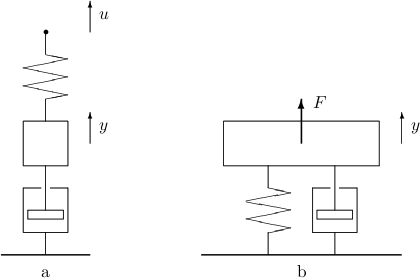
\includegraphics[width=6cm]{./bilder/federkrafterregung.png}}
	& \begin{minipage}[]{12cm}
      \renewcommand{\arraystretch}{2}      
		\begin{tabular}{ll}
    	Differentialgleichung
    		& $m \, \ddot{y} + b \, \dot{y} + c y=$
    		\textcolor{blue}{$\underbrace{c\,u_0}_{F_0} \, \sin(\omega t)$} \\
    	Amplitude
    		&
    		$A=\dfrac{c\,u_0}{m\sqrt{(\omega_0^2-\omega^2)^2+(2D\,\omega_0\,\omega)^2}}$ \\
    	Phase zw. $\omega_0$ \& $\omega$
    		&
    		$\varphi=\arctan\left(\dfrac{2D\,\omega_0\,\omega}{\omega_0^2-\omega^2}\right)$\\ 
    	Resonanzkreisfrequenz
    		& $\omega_r=\omega_0\sqrt{1-2D^2}$\quad $\omega_r<\omega_d<\omega_0$\\
    	Resonanzamplitude
    		& $A_r=\dfrac{u_0}{2D\sqrt{1-D^2}} = \dfrac{c \cdot u_0}{2m\sqrt{(\delta \omega_0)^2 - \delta^4}}$\\
    	Vergrösserungsfunktion
    		&
    		$V=\dfrac{1}{\sqrt{(1-\eta^2)^2+(2D\eta)^2}}=\dfrac{A(\omega)}{u_0}$ \\ 
    	Vergrösserung bei Resonanz
    		&
    		$V_r = \dfrac{1}{\sqrt{1-\eta_r^4}}$ mit $\eta_r = \sqrt{1-2D^2}$\\
    	\multicolumn{2}{l}{\parbox{12cm}{\small
    	Überkritische Dämfpung, wenn $D > \frac{1}{\sqrt2} \Rightarrow$ Auch bei 
    	Resonanz\\
    	bleibt Amplitude stets unter statischer
    	Auslenkung ($V \leq 1$)}}
		\end{tabular}
    \end{minipage} \\
\hline
\parbox{6cm}{
	\textbf{Unwuchterregung}\\ \\
	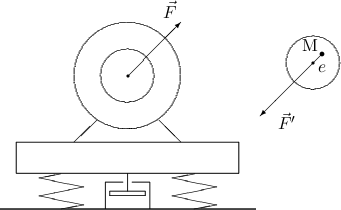
\includegraphics[width=6cm]{./bilder/unwuchterregung.png}\\ \\
	$m_R$ Rotormasse (bewegt)\\
	$e$ Exzentrizit"at (Distanz Achse$\leftrightarrow$SP) \\
	$F_0$ Kraft auf Fundament ohne Federung\\
	$F_{B0}$ verringerte Kraft}
	& \begin{minipage}[]{12cm}
      \renewcommand{\arraystretch}{2}
		\begin{tabular}{ll}
        $F(t)=F_0\cdot\sin(\omega t)$
        	& $F_0=m\cdot a_r=m\cdot\dfrac{v^2}{r}=m\cdot r\cdot \omega^2=m_R\cdot e \cdot \omega^2$ \\
    	Differentialgleichung
    		& $m\,\ddot{y}+b\,\dot{y}+c\,y=$
    		\textcolor{blue}{$m_R\,e\,\omega^2\,\sin(\omega t)$} \\
    	Amplitude
    		&
    		$A=\dfrac{m_R\,e\,\omega^2}{m\sqrt{(\omega_0^2-\omega^2)^2+(2D\,\omega_0\,\omega)^2}}$ \\
    	Phase zw. $\omega_0$ \& $\omega$
    		&
    		$\varphi=\operatorname{arctan}\left(\dfrac{2D\,\omega_0\,\omega}{\omega_0^2-\omega}\right)$\\ 
    	Resonanzkreisfrequenz
    		& $\omega_r=\dfrac{\omega_0}{\sqrt{1-2D^2}}$\\
    	Resonanzamplitude
    		& $A_r=\dfrac{m_R}{m}\dfrac{e}{2D\sqrt{1-D^2}}$\\
    	Kraftamplitude \textbf{ohne} Fed.
    		& $F_0 = m_R\,e\,\omega^2 \sin(\omega t)$\\
		Kraftamplitude \textbf{mit} Fed.
    		&
    		$F_{B0}=\dfrac{m_R\,e\,\omega^2\,\sqrt{1+4D^2\eta^2}}{\sqrt{(1-\eta^2)^2+4D^2\eta^2}}=F(\eta)$ \\ 
    	Verhältnis
    		&$\dfrac{F_{B0}}{F_0}=\sqrt{\dfrac{1+4D^2\eta^2}{(1-\eta^2)^2+4D^2\eta^2}}$ \\ 
		\end{tabular}
    \end{minipage} \\
\hline
\parbox{6cm}{
	\textbf{Indirekte Federkrafterregung}\\
	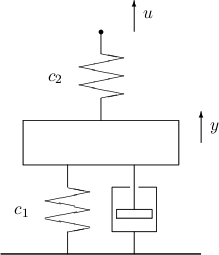
\includegraphics[width=4cm]{./bilder/indirekte-federkrafterregung.png}}
	& \begin{minipage}[]{12cm}
      \renewcommand{\arraystretch}{2}
		\begin{tabular}{ll}
    	Differentialgleichung
    		& $m \, \ddot{y} + b \, \dot{y} + c y=$
    		\textcolor{blue}{$c_2 \, u_0 \, \sin(\omega t)$} \\
    	Amplitude
    		&
    		$A=\dfrac{c_2}{c} 
    		\dfrac{c\,u_0}{m\sqrt{(\omega_0^2-\omega^2)^2+(2D\,\omega_0\,\omega)^2}}$ \\
    	Phase zw. $\omega_0$ \& $\omega$
    		&
    		$\varphi=\arctan\left(\dfrac{2D\,\omega_0\,\omega}{\omega_0^2-\omega^2}\right)$\\ 
    	Resonanzkreisfrequenz
    		& $\omega_r=\omega_0\sqrt{1-2D^2}$\\
    	Resonanzamplitude
    		& $A_r=\dfrac{u_0}{2D\sqrt{1-D^2}}$\\
    	Vergrösserungsfunktion
    		&
    		$V=\dfrac{c_2}{c}\cdot\dfrac{1}{\sqrt{(1-\eta^2)^2+(2D\eta)^2}}$
		\end{tabular}
    \end{minipage} \\
\hline
\end{tabular}

\renewcommand{\arraystretch}{1.3}
\begin{tabular}{|l|l|}
\hline
\parbox{6cm}{
	\textbf{Stützenerregung}\\ \\
	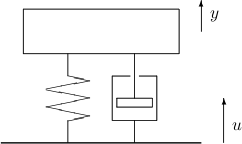
\includegraphics[width=4cm]{./bilder/stuetzenerregung.png}}
	& \begin{minipage}[]{12cm}
      \renewcommand{\arraystretch}{2}
		\begin{tabular}{ll}
    	Differentialgleichung
    		& $m\,\ddot{y}+b\,\dot{y}+c\,y=$
    		\textcolor{blue}{$c\,u_0\,\sin(\omega t) + b\,\omega\,u_0\,\cos(\omega t)$}
    		\\ & $m\, \ddot{q} + b\,\dot{q} + c\,q =$
    		\textcolor{blue}{$m\,\omega^2\,u_0\,\sin(\omega t)$} \\
    	Amplitude
    		&
    		$A=\dfrac{\omega^2\,u_0}{\sqrt{(\omega_0^2-\omega^2)^2+(2D\,\omega_0\,\omega)^2}}$ \\
    	Phase zw. $\omega_0$ \& $\omega$
    		&
    		$\varphi=\arctan\left(\dfrac{2D\,\omega_0\,\omega}{\omega_0^2-\omega^2}\right)-\pi$\\ 
    	Resonanzkreisfrequenz
    		& $\omega_r=\dfrac{\omega_0}{\sqrt{1-2D^2}}$\\
    	Resonanzamplitude
    		& $A_r=\dfrac{u_0}{2D\sqrt{1-D^2}}$\\
    	Vergrösserungsfunktion
    		& $V=\dfrac{\eta^2}{\sqrt{(1-\eta^2)^2+(2D\eta)^2}}$ 
		\end{tabular}
    \end{minipage} \\
\hline
\parbox{6cm}{
	\textbf{Dämpferregung}\\ \\
	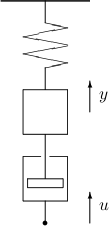
\includegraphics[width=2cm]{./bilder/daempferregung.png}}
	& \begin{minipage}[]{12cm}
      \renewcommand{\arraystretch}{2}
		\begin{tabular}{ll}
    	Differentialgleichung
    		& $m\,\ddot{y}+b\,\dot{y}+c\,y=$
    		\textcolor{blue}{$b\,\omega\,u_0\,\sin(\omega t+\frac{\pi}{2})$} \\
    	Amplitude
    		&
    		$A=\dfrac{b\,\omega\,u_0}{m\sqrt{(\omega_0^2-\omega^2)^2+(2D\,\omega_0\,\omega)^2}}$ \\
    	Phase zw. $\omega_0$ \& $\omega$
    		&
    		$\varphi=\operatorname{arctan}\left(\dfrac{2D\,\omega_0\,\omega}{\omega_0^2-\omega^2}\right)-\dfrac{\pi}{2}$\\ 
    	Resonanzkreisfrequenz
    		& $\omega_r=\omega_0 \quad \rightarrow$\quad max. bei $\eta=1$\\
    	Resonanzamplitude
    		& $A_r=u_0\quad\rightarrow\quad V(1)=1$\\
    	Vergrösserungsfunktion
    		&
    		$V=\dfrac{2 \,D\, \eta}{\sqrt{(1-\eta^2)^2+(2D\eta)^2}}$ 
		\end{tabular}
    \end{minipage} \\
\hline
\end{tabular}
\renewcommand{\arraystretch}{1}
%\newpage
\subsection{Elektrische Schwingkreise \kuchling{530} \stoecker{253}}
\renewcommand{\arraystretch}{1.5}
\begin{tabular}{|p{4cm}|p{7cm}|p{7cm}|}
\hline
& Serienschwingkreis & Parallelschwingkreis\\
\hline
Diffgl: &
\begin{minipage}[]{7cm}
\vspace{0.2cm}
$L\ddot{I}+R_S\dot{I}+\dfrac{1}{C}\,I=\omega\,U_0\,\sin(\omega t + \dfrac{\pi}{2})$ \qquad 
%$I=I_0\,e^{-\delta t}\,\sin(\omega_d t+\varphi)$\\
\end{minipage} &
\begin{minipage}[]{7cm}
\vspace{0.2cm}
$C\ddot{U}+\dfrac{1}{R_P}\dot{U}+\dfrac{1}{L}U=\omega\,I_0\,\sin(\omega
t+\dfrac{\pi}{2})$\\
\end{minipage}
\\
\hline
Amplitude: &
\begin{minipage}[]{7cm}
\vspace{0.1cm}
$I_0=\dfrac{\omega\,U_0}{L\sqrt{(\omega_0^{\,2}-\omega^2)^2+(2D\,\omega_0\,\omega)^2}}$\\
\end{minipage} &
\begin{minipage}[]{7cm}
\vspace{0.1cm}
$U_0=\dfrac{\omega\,I_0}{C\sqrt{(\omega_0^{\,2}-\omega^2)^2+(2D\,\omega_0\,\omega)^2}}$\\
\end{minipage}\\
\hline
Phase: &
\begin{minipage}[]{7cm}
\vspace{0.1cm}
$\varphi=\arctan \left( {\dfrac{2D\,\omega_0\,\omega}{\omega_0^{\,2}-\omega^2}}\right) -\dfrac{\pi}{2}$\\
\end{minipage}&
\begin{minipage}[]{7cm}
\vspace{0.2cm}
$\varphi=\arctan\left( {\dfrac{2D\,\omega_0\,\omega}{\omega_0^{\,2}-\omega^2}}\right) -\dfrac{\pi}{2}$\\
\end{minipage}\\
\hline
Resonanzfrequenz: &
\begin{minipage}[]{7cm}
\vspace{0.1cm}
$\omega_r=\omega_0=\dfrac{1}{\sqrt{LC}}$ \qquad
$\omega_d=\omega_0\sqrt{1-D^2}
%=\dfrac{1}{\sqrt{LC}}\,\sqrt{1-\dfrac{R^2C}{4L}}
$ \end{minipage}
&
\begin{minipage}[]{7cm}
\vspace{0.2cm}
$\omega_r=\omega_0=\dfrac{1}{\sqrt{LC}}$\\
\end{minipage}\\
\hline
Resonanzamplitude: &
\begin{minipage}[]{7cm}
\vspace{0.1cm}
$I_{0_r}=\dfrac{U_0}{R_S}$\\
\end{minipage}&
\begin{minipage}[]{7cm}
\vspace{0.2cm}
$U_{0_r}=I_0\cdot R_P\qquad$ mit $ R_P =\dfrac{\omega^2\,L^2}{R_S}$\\
\end{minipage}\\
\hline
Vergr"osserungsfunktion: &
\begin{minipage}[]{7cm}
\vspace{0.1cm}
$V(\eta)=\dfrac{\eta^2}{\sqrt{(1-\eta^2)^2+(2D\,\eta)^2}}$\\ Max:
$V_m=\dfrac{1}{2D\sqrt{1-D^2}}$\\
\end{minipage} &
\begin{minipage}[]{7cm}
\vspace{0.2cm}
$V(\eta)=\dfrac{1}{\sqrt{(1-\eta^2)^2+(2D\,\eta)^2}}$\\
Max: $V_m=\dfrac{1}{2D\sqrt{1-D^2}}$\\
\end{minipage}\\
\hline
Phasenverschiebung: &
\begin{minipage}[]{7cm}
\vspace{0.1cm}
$\varphi_{_U}=\arctan\left(\dfrac{2D\,\eta}{1-\eta^2}\right)-\pi$\\
\end{minipage} &
\begin{minipage}[]{7cm}
\vspace{0.2cm}
$\varphi_{_I}=\arctan\left(\dfrac{2D\,\eta}{1-\eta^2}\right)$\\
\end{minipage}\\
\hline
D"ampfungsgrad: &
\begin{minipage}[]{7cm}
\vspace{0.1cm}
$D=\dfrac{R_S}{2}\sqrt{\dfrac{C}{L}}$\\
\end{minipage} &
\begin{minipage}[]{7cm}
\vspace{0.2cm}
$D=\dfrac{1}{2\,R_P}\sqrt{\dfrac{L}{C}}$\\
\end{minipage}\\
\hline
%Abklingkonst. : &
%\begin{minipage}[]{7cm}
%\vspace{0.2cm}
%$\delta=\dfrac{R_S}{2L}$\\
%\end{minipage}\\
%\hline
\end{tabular}

\subsubsection{G"ute}
$Q=2\pi\dfrac{E(t)}{E(t)-E(t+T)}=\dfrac{1}{2D}=V_m=\dfrac{\omega_0}{\Delta \omega}$\quad wobei \quad $E=\dfrac{C\,U^2}{2}+\dfrac{L\,I^2}{2}=\dfrac{L\,I_0^{\,2}}{2}=\dfrac{L\,\omega_0^{\,2}\,C^2\,U_0^{\,2}}{2}=\dfrac{C\,U_0^{\,2}}{2}$
